\chapter{أنشئ أنواع متغيرات خاصّة بك}

تسمح لغة الـ\textenglish{C}
بالقيام بشيء يعتبر قوياً جداً : و هو أن ننشئ أنواعاً خاصة بنا، "أنواع متغيّرات مخصّصة". سنرى نوعين : الـهياكل
(\textenglish{Structures})
و التعدادات
(\textenglish{Enumerations}).

 إن إنشاء أنواع خاصّة بنا يعتبر أمراً ضروريا خاصة إذا أردنا إنشاء برامج أكثر تعقيداً.

الأمر ليس  (لحسن الحظّ) بالصعب، لكن ركّز جيّدا لأننا سنستعمل الهياكل كل الوقت انطلاقا من الفصل القادم.\\
يجب أن تعلم أنّ المكتبات تنشئ غالبا أنواعها الخاصّة. لن يمرّ وقت كثير حتّى تستخدم نوعا يدعى "ملف"، و بعده بقليل، أنواع أخرى مثل "نافذة"، "صوت"، "لوحة مفاتيح"، إلخ.

\section{تعريف هيكل}

الهيكل هو تجميع لعدد من المتغيرات التي يمكن لها أن تحمل أنواعا مختلفة. على عكس الجداول التي ترغمنا على استعمال خانات من نفس النوع في كلّ الجدول، بإمكانك تعريف هيكل يحمل الأنواع :
\InlineCode{long}، \InlineCode{char}، \InlineCode{int}
و
\InlineCode{double}
في مرّة واحدة.

الهياكل في أغلب الأحيان معرّفة في ملفات
\InlineCode{.h}
مثلما رأينا مع
\InlineCode{\#define}
و نماذج الدوال. هذا مثال عن هيكل :

\begin{Csource}
struct StructureName
{
	int variable1;
	int variable2;
	int anotherVariable;
	double decimalNumber;
};
\end{Csource}

لتعريف هيكل، يجب علينا أن نبدأ بالكلمة المفتاحية
\InlineCode{struct}،
متبوعة باسم الهيكل (مثلا
\InlineCode{File}
أو
\InlineCode{Screen}).

\begin{information}
  شخصيّا لديّ عادة في تسمية هياكلي بنفس قواعد تسمية المتغيّرات، باستثناء أنّي أجعل أوّل حرف كبيرا للتفريق. هكذا، عندما أرى الكلمة
\InlineCode{captainAge}
في شفرتي، أعلم أنّها متغيّر لأنّها تبدأ بحرف صغير. عندما أرى
\InlineCode{AudioPart}
فأعلم أنّها هيكل (نوع مخصّص) لأنّها تبدأ بحرف كبير.
\end{information}

بعد ذلك، نفتح حاضنة لنغلقها لاحقاً تماما مثل الدوال.

\begin{critical}
  احذر، الأمر خاصّ هنا : بالنسبة للهياكل، يجب أن تضع بعد الحاضنة النهائية فاصلة منقوطة. هذا أمر إجباري. إن لم تفعله فستتوقّف الترجمة.
\end{critical}

و الآن، ماذا نضع داخل الحاضنتين ؟\\
هذا سهل، سنضع المتغيرات التي يتكون منها الهيكل، و عادة ما يتكون الهيكل من "مُتَغَيِّريْن داخِلِيَيْن" على الأقل، و إلا فلن يحمل معنى كبيرا.

كما ترى، فإنشاء نوع متغيّرات مخصّص ليس بالأمر الصعب. كلّ الهياكل ماهي إلّا "تجميعات" لمتغيّرات من أنواع قاعديّة مثل
\InlineCode{long}، \InlineCode{int}، \InlineCode{double}،
إلخ. لا توجد معجزة، إنّ نوعا
\InlineCode{File}
مثلاً ما هو إلا مجموعة من الأعداد القاعديّة !

\subsection{مثال عن هيكل}

تخيل أنك تريد إنشاء متغيّر لكي يٌخزّن إحداثيات نقطة في معلم الشاشة. ستحتاج بالتأكيد إلى هيكل كهذا عندما تبدأ في برمجة ألعاب ثنائية الأبعاد في الجزء التالي من الكتاب، هذه إذن فرصة للتقدّم قليلا.

إذا كانت كلمة "علم الهندسة" تُحدث ظهور بُقَع غير مفهومة على كامل وجهك، فالمخطّط التالي سيذكّرك قليلا بأساسيّات الأبعاد الثنائيّة (\textenglish{2D}).

\begin{figure}[H]
	\centering
	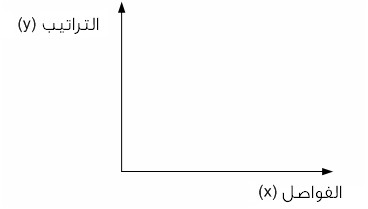
\includegraphics[width=0.4\textwidth]{Chapter_II-6_Axis}
\end{figure}

عندما نعمل في
\textenglish{2D}
لدينا محوران : محور الفواصل (من اليسار إلى اليمين) و محور التراتيب (من الأسفل إلى الأعلى). من العادة أن نرمز للفواصل بمتغيّر يدعى
\InlineCode{x}
و للتراتيب بـ\InlineCode{y}.

هل يمكنك كتابة هيكل
\InlineCode{Coordinates}
يسمح بتخزين كلّا من الفاصلة
(\InlineCode{x})
و الترتيبة
(\InlineCode{y})
لنقطة ما~؟\\
هيّا، هيّا، الأمر ليس صعبا :

\begin{Csource}
struct Coordinates
{
	int x; // Abscissas
	int y; // Ordinates
};
\end{Csource}

هيكلنا يسمّى
\InlineCode{Coordinates}
و هو متكوّن من متغيرين
\InlineCode{x}
و
\InlineCode{y}
أي الفاصلة
(\textenglish{Abscissa})
و الترتيبة
(\textenglish{Ordinate}).

إن أردنا، يمكننا بسهولة إنشاء هيكل
\InlineCode{Coordinates}
من أجل
\textenglish{3D} :
يكفي فقط إضافة متغيّر ثالث (مثلا
\InlineCode{z})
يدلّ على الارتفاع. بهذا سيكون لدينا هيكل لإدارة النقاط الثلاثيّة الأبعاد في الفضاء~!

\subsection{جدول داخل هيكل}

يمكن للهياكل أن تحتوي على جداول. هذا جيّد، إذ يمكننا أن نضع داخلها جداول
\InlineCode{char}،
(سلاسل محرفيّة) بدون أيّة مشاكل.\\
فلنتخيل هيكلاً
\InlineCode{Person}
و الذي يحتوي على معلومات عن شخص :

\begin{Csource}
struct Person
{
	char firstName[100];
	char lastName[100];
	char address[1000];
	int age;
	int boy; // Boolean : 1 = boy, 0 = girl
};
\end{Csource}

هذا الهيكل متشكّل من 5 متغيرات داخليّة، الثلاث الأولى هي سلاسل محرفيّة لتخزين الاسم، اللقب و العنوان.\\
المتغيران الأخيران يخزّنان عُمر و جنس الشخص. الجنس هو متغيّر منطقي، 1 = صحيح = ولد و 0 = خطأ = بنت.

يمكن لهذا الهيكل أن يساعدنا في كتابة برنامج مذكّرة عناوين. يمكنك بالطبع إضافة القدر الذين تريد من المتغيرات داخل الهيكل من أجل إتمامها إذا أردت. لا يوجد حدّ لعدد المتغيّرات في هيكل.

\section{استعمال هيكل}

و الآن، بما أن الهيكل معرّف في ملف
\InlineCode{.h}،
سنتمكّن من استعماله في دالة موجودة بملف
\InlineCode{.c}.\\
أنظر كيف نقوم بإنشاء متغير من نوع
\InlineCode{Coordinates}
(الهيكل الّذي عرّفناه سابقا) :
\begin{Csource}
#include "main.h" // Including the files that contains the prototypes and structures
int main(int argc, char *argv[])
{
	struct Coordinates point; // Creating a variable "point" of type Coordinates
	return 0;
}
\end{Csource}
هكذا نكون قد أنشأنا متغيراً
\InlineCode{point}
من نوع
\InlineCode{Coordinates} !
هذا المتغير سيحمل داخله مركّبين (متغيرين داخليين) :
\InlineCode{x}
و
\InlineCode{y}
(فاصلته و ترتيبته).

\begin{question}
  هل من اللازم أن نضع الكلمة المفتاحية
\InlineCode{struct}
عند تعريف المتغير ؟
\end{question}

نعم، فهذا يسمح للحاسوب بأن يفرّق بين نوع عادي (مثل
\InlineCode{int})
و نوع مخصّص.\\
المبرمجون وجدوا أنه من المتعب جدّا أن يكتبوا في كلّ مرة الكلمة
\InlineCode{struct}
في كلّ تعريف لمتغيّر مخصّص.
لمعالجة هذا المشكل، اخترعوا تعليمة خاصّة : الـ\InlineCode{typedef}.

\subsection{الـ\texttt{typedef}}

لنعد إلى الملف
\InlineCode{.h}
الذي يحمل تعريف هيكلنا من نوع
\InlineCode{Coordinates}.
سنضيف تعليمة اسمها
\InlineCode{typedef}
و الّتي تفيد في إعطاء اسم مستعار
(\textenglish{alias})
لهيكل، أي كتابة شيء مكافئ لكتابة آخر.

إذا، سنضيف سطرا يبدأ بـ\InlineCode{typedef}
قبل تعريف الهيكل مباشرة :

\begin{Csource}
typedef struct Coordinates Coordinates;
struct Coordinates
{
	int x;
	int y;
};
\end{Csource}

هذا السطر متكون من ثلاثة أجزاء :

\begin{itemize}
  \item \InlineCode{typedef} :
  تعني أننا سنقوم بإنشاء اسم مستعار لهيكل.
  \item \InlineCode{struct Coordinates} :
  هو اسم الهيكل الذي سنقوم بانشاء اسم مستعار له (أي "مكافئ").
  \item \InlineCode{Coordinates} :
  هو الاسم المكافئ.
\end{itemize}

ببساطة، هذا السطر يقول : "كتابة
\InlineCode{Coordinates}
مكافئ لكتابة
\InlineCode{struct Coordinates}".
بفعل هذا، لن يكون عليك كتابة الكلمة
\InlineCode{struct}
عند كلّ تعريف لمتغيّر من نوع
\InlineCode{Coordinates}.
يمكننا العودة إلى
\InlineCode{main}
و كتابة فقط :

\begin{Csource}
int main(int argc, char *argv[])
{
	 Coordinates point; // The computer understands that we are talking about "struct Coordinates" thanks to typedef
   return 0;
}
\end{Csource}

أنصحك أن تستعمل الـ\InlineCode{typedef}
مثلما فعلت أنا هنا من أجل
\InlineCode{Coordinates}.
أغلب المبرمجين يفعلون هذا. هذا يسمح لهم بعدم كتابة
\InlineCode{struct}
في كلّ مرّة. المبرمج الجيّد هو مبرمج كسول ! أي أنه يكتب أقل ما يمكن.

\subsection{تغيير مركّبات هيكل}

و الآن بعدما قمنا بإنشاء متغيّرنا
\InlineCode{point}،
نريد أن نغيّر إحداثيّاته.\\
كيف نصل إلى
\InlineCode{x}
و
\InlineCode{y}
الموجودة في المتغير
\InlineCode{point}
؟ هكذا :

\begin{Csource}
int main(int argc, char *argv[])
{
	Coordinates point;
	point.x = 10;
	point.y = 20;
	return 0;
}
\end{Csource}

بهذا نكون قد غيّرنا قيمة
\InlineCode{point}،
بإعطائه الفاصلة 10 و الترتيبة 20. نقطتنا أصبحت في الوضعية (10؛20) (هذا هو الترميز الرياضياتي للإحداثيّات).

لكي نتمكن من الوصول إلى مركّب في الهيكل، يجب كتابة :

\begin{Csource}
  variable.componentName
\end{Csource}

النقطة هي التي تفرّق بين المتغير و المركّب.

إن أخذنا الهيكل
\InlineCode{Person}
الذي رأيناه منذ قليل و نطلب الاسم و اللقب فسنفعل هكذا :

\begin{Csource}
int main(int argc, char *argv[])
{
	Person user;
	printf("What's your last name ? ");
	scanf("%s", user.lastName);
	printf("What's your first name ? ");
	scanf("%s", user.firstName);
	printf("You are %s %s", user.firstName, user.lastName);
	return 0;
}
\end{Csource}

\begin{Console}
What's your last name ? Dupont
What's your first name ? Jean
You are Jean Dupont
\end{Console}

نرسل المتغير
\InlineCode{user.lastName}
إلى الدالة
\InlineCode{scanf}،
و التي ستكتب مباشرة في
\InlineCode{user}.\\
نفعل نفس الشيء مع
\InlineCode{firstName}،
يمكننا فعل ذلك أيضا مع العنوان، العمر و الجنس، لكنّي لا أرغب بتكرار ذلك (يحب أن أكون مبرمجا !).

يمكن فعل هذا بدون معرفة الهياكل، فقط بإنشاء متغيّر
\InlineCode{lastName}
و آخر
\InlineCode{firstName}.\\
لكن الفائدة هنا هي أنه بهذه الطريقة يمكننا أن ننشئ متغيرا آخر من نوع
\InlineCode{Person}
و يكون لديه هو أيضا اسمه الخاص، لقبه الخاص، إلخ. يمكننا إذن فعل هذا :

\begin{Csource}
Person player1, player2;
\end{Csource}

و هكذا نخزّن معلومات كلّ لاعب. كلّ لاعب سيكون لديه اسمه الخاص، لقبه الخاص، إلخ.

يمكننا أن نفعل ما هو أفضل : يمكننا تعريف جدول من
\InlineCode{Person} !\\
القيام بهذا سهل :

\begin{Csource}
Person players[2];
\end{Csource}

و بعدها يمكننا الوصول إلى لقب اللاعب المتواجد بالخانة الأولى مثلا، هكذا :

\begin{Console}
players[0].lastName
\end{Console}

الفائدة من استعمال الجدول هنا، هو أنها بامكاننا استعمال حلقة لنقرأ المعلومات الخاصة باللاعب 1 و اللاعب 2 بدون الاضطرار إلى إعادة الشفرة مرّتين. يكفي تصفّح الجدول
\InlineCode{players}
و طلب كلّ مرّة اللقب، الاسم، العنوان \dots

\paragraph{تمرين :}
قم بتعريف جدول من نوع
\InlineCode{Person}،
و اقرأ المعلومات الخاصة بكلّ لاعب باستخدام حلقة. إبدأ بجدول ذي خانتين، و إن كان ذلك ممتعا، حاول تكبير العدد لاحقا.\\
في النهاية، عليك بإظهار المعلومات التي أخذتها من كلّ لاعب.

\subsection{تهيئة هيكل}

بالنسبة للهياكل، مثل كلّ المتغيرات، الجداول و المؤشّرات، فنحن نفضّل أن نعطيها قيما ابتدائية كي نضمن أنّها لن تحوي "قيما عشوائية". في الواقع، أعيد تذكيرك، المتغير الّذي يتمّ إنشائه يأخذ القيمة الموجودة في الذاكرة حيث تمّ وضعه. أحيانا تكون هذه القيمة $ 0 $، و أحيانا بقايا برنامج مرّ قبلك، لذلك ستكون قيمته شيئا لا معنى له، مثل
$-84570$.

للتذكير، هكذا نقوم بالتهيئة :

\begin{itemize}
  \item  المتغير : نعطيه القيمة 0 (الحالة الأبسط).
  \item المؤشّر : نجعل قيمته
\InlineCode{NULL}.
بالمناسبة فـ\InlineCode{NULL}
هي
\InlineCode{\#define}
موجود في مكتبة
\InlineCode{stdlib.h}
و هي عادة 0، لكنّنا نستمرّ في استخدام
\InlineCode{NULL}
للمؤشرات لكي نبيّن أنّها مؤشّرات و ليست متغيّرات عاديّة.
  \item الجدول : نضع كلّ خاناته على القيمة 0.
\end{itemize}

بالنسبة للهياكل، فالتهيئة شبيهة بتلك الخاصّة بالجدول. في الواقع، يمكننا القيام بها عند التصريح عن المتغيّر :

\begin{Csource}
Coordinates point = {0, 0};
\end{Csource}

و هذا يعرّف بالترتيب :
\InlineCode{point.x = 0}
و
\InlineCode{point.y = 0}.
لنعد إلى الهيكل
\InlineCode{Person}
(الذي يحتوي سلاسل محرفيّة). يمكننا أن نعطي قيمة ابتدائية للسلاسل بكتابة فقط
\InlineCode{""}
(لا شيء ببن علامتي الاقتباس). لم أعلمك هذا الشيء في الفصل الخاصّ بالسلاسل، لكنّ الوقت ليس متأخّرا على تعلّمها.
يمكننا إذن تهيئة على الترتيب
\InlineCode{firstName}،
\InlineCode{lastName}،
\InlineCode{address}،
\InlineCode{age}،
و
\InlineCode{boy}
هكذا :

\begin{Csource}
Person user= {"", "", "", 0, 0};
\end{Csource}

رغم ذلك، أنا لا أستخدم هذه التقنيّة كثيرا. أفضّل أن أرسل متغيّري، مثلا
\InlineCode{point}،
إلى دالّة
\InlineCode{initializeCoordinates}
تقوم بالتهيئات من أجلي على متغيري.\\
لفعل هذا، يجب إرسال مؤشّر نحو متغيري. في الواقع، إن أرسلت فقط المتغيّر، سيتم إنشاء نسخة عنه (مثل أيّ متغيّر عادي) و تعديل قيم النسخة لا قيم المتغيّر. راجع الخيط الأحمر من فصل المؤشرات إن نسيت كيف يعمل هذا الأمر.

يجب إذن تعلّم كيفيّة استخدام المؤشرات على الهياكل. الأمور بدأت تصعب قليلا !

\section{مؤشّر نحو هيكل}

المؤشّر على الهيكل يتمّ إنشائه بنفس طريقة إنشاء مؤشّر على
\InlineCode{int}
أو
\InlineCode{double}
أو أيّ نوع قاعديّ آخر :

\begin{Csource}
Coordinates* point = NULL;
\end{Csource}
بهذا نكون قد عرّفنا مؤشّرا نحو
\InlineCode{Coordinates}
اسمه
\InlineCode{point}.\\
و لأن التذكير لن يضرّ أحدا، أعيد إخبارك بأنه من الممكن وضع النجمة أمام اسم المتغيّر، فهذه الكتابة مكافئة تماما للسابقة~:

\begin{Csource}
Coordinates *point = NULL;
\end{Csource}

أنا أفعل هكذا كثيرا، لأنه لتعريف عدّة مؤشرات على سطر واحد، سيكون علينا وضع النجمة أمام اسم كل واحد منها :

\begin{Csource}
Coordinates *point1 = NULL, *point2 = NULL;
\end{Csource}

\subsection{إرسال هيكل إلى دالة}

الشيء الذي يهمّنا هنا، هو كيفيّة إرسال مؤشر هيكل إلى دالة كي تقوم هذه الأخيرة بتعديل محتواه.

هذا ما سنقوم به في هذا المثال، سنقوم بإنشاء متغير من نوع
\InlineCode{Coordinates}
في
\InlineCode{main}،
و نرسل عنوانه إلى
\InlineCode{initializeCoordinates}.
دور هذه الدالة هو إعطاء القيمة 0 لعناصر الهيكل.

دالتنا
\InlineCode{initializeCoordinates}
ستأخذ معاملا واحدا : مؤشر نحو هيكل من نوع
\InlineCode{Coordinates}
(أي
\InlineCode{*Coordinates}).

\begin{Csource}
int main(int argc, char *argv[])
{
	Coordinates myPoint;
	initializeCoordinates(&myPoint);
	 return 0;
}
void initializeCoordinates(Coordinates* point)
{
	// Initializing each member of the structure here
}
\end{Csource}

متغيري
\InlineCode{myPoint}
تم إنشاؤه في
\InlineCode{main}.\\
نقوم يارسال عنوانه إلى الدالة
\InlineCode{initializeCoordinates}
الّتي تسترجعه على شكل متغيّر يسمّى
\InlineCode{point}
(كان بإمكاننا تسميته كما شئنا، هذا الأمر ليس له أيّ تأثير).

الآن بما أنّنا داخل الدالة
\InlineCode{initializeCoordinates}،
سنقوم يتهيئة قيم المتغير
\InlineCode{point}
واحدة بواحدة.\\
يجب عدم نسيان وضع النجمة أمام اسم المؤشر للوصول إلى المتغير. إن لم تفعل، فأنت تخاطر بتغيير العنوان، و ليس هذا ما نريد فعله.

و لكن هاهي مشكلة \dots لا يمكننا القيام مباشرة بهذا :

\begin{Csource}
void initializeCoordinates(Coordinates* point)
{
	*point.x = 0;
	*point.y = 0;
}
\end{Csource}

سيكون ذلك سهلا جدّا \dots لماذا لا يمكننا القيام بهذا ؟
لأنّ النقطة تطبّق على
\InlineCode{point}
فقط و ليس على
\InlineCode{*point}.
لكنّ ما نريده هو الوصول إلى
\InlineCode{*point}
لتغيير قيمته.\\
لحلّ هذا المشكل، يجب وضع الأقواس حول
\InlineCode{*point}،
هكذا ستطبّق النقطة على
\InlineCode{*point}
و ليس فقط على
\InlineCode{point} :

\begin{Csource}
void initializeCoordinates(Coordinates* point)
{
	(*point).x = 0;
	(*point).y = 0;
}
\end{Csource}

هذه الشفرة تعمل، يمكنك تجريبها. المتغير من نوع
\InlineCode{Coordinates}
تمّ إرساله إلى الدالة التي هيّأت
\InlineCode{x}
و
\InlineCode{y}
على 0.

\begin{information}
في لغة الـ\textenglish{C}،
نهيّئ عادة هياكلنا بالطريقة الّتي رأيناها سابقا. بالمقابل، في لغة الـ\textenglish{C++}،
التهيئة تكون في الغالب داخل "دوال".
إن لغة
\textenglish{C++}
ليست سوى "تحسين خارق" للهياكل. كثير من الأشياء تبدأ من هذا و أحتاج إلى كتاب كامل لأتحدّث عنها (كلّ شيء في وقته).
\end{information}

\subsection{اختصار عمليّ و مستعمل بكثرة}

سترى أننا سنستعمل كثيراً مؤشرات نحو هياكل. بصراحة، يجب أن أعترف لك بأنّه
في لغة الـ\textenglish{C}
نستخدم  المؤشرات نحو الهياكل أكثر من استعمال الهياكل وحدها. لهذا فعندما أقول لك بأنّ المؤشرات ستظلّ تتبعك حتّى إلى قبرك، فأنا لا أقولها تقريبا من أجل المزاح !

بما أن المؤشرات نحو الهياكل مستعملة بكثرة، نجد أنفسنا نستعمل هذه الكتابة كثيرا :
\begin{Csource}
(*point).x = 0;
\end{Csource}

مرّة أخرى، المبرمجون وجدوا هذه الكتابة طويلة جدّا. الأقواس حول
\InlineCode{*point}،
يا لها من بلوى~! إذن، بما أن المبرمجين أشخاص كسالى (لقد قلت هذا سابقا على ما أعتقد)، فقد اخترعوا هذا الاختصار :

\begin{Csource}
point->x = 0;
\end{Csource}

هذا الاختصار يتمّ كتابته بمطّة
\InlineCode{-}
متبوعة بعلامة ترتيب
\InlineCode{>}.

كتابة
\InlineCode{point->x}
هو إذن مكافئ
\underline{تماما}
لكتابة
\InlineCode{(*point).x}.

\begin{warning}
  لا تنس أننا لا نستطيع استعمال السهم إلا مع المؤشرات.\\
إن كنت تعمل على المتغير مباشرة، يجب عليك استخدام النقطة كما رأينا في البداية.
\end{warning}

لنعد إلى دالتنا
\InlineCode{initializeCoordinates}
يمكننا كتابتها بالشكل التالي :

\begin{Csource}
void initializingCoordinates(Coordinates* point)
{
	point->x = 0;
	point->y = 0;
}
\end{Csource}

و تذكّر جيّدا اختصار السهم، سنستعمله كثيراً من الآن. و خاصّة لا تخلط بين السهم و "النقطة". السهم مخصّص للمؤشّرات، "النقطة" مخصّصة للمتغيّرات. استخدم هذا المثال الصغير للتذكّر :

\begin{Csource}
int main(int argc, char *argv[])
{
	Coordinates  myPoint;
	Coordinates *pointer = &myPoint;
	myPoint.x = 10; // We work on a variable, we use the "dot"
	pointer->x = 10; // We work on a pointer, we use the arrow
	return 0;
}
\end{Csource}

نغيّر قيمة
\InlineCode{x}
إلى 10 بطريقتين مختلفتين، هنا : الطريقة الأولى هي بالعمل مباشرة على المتغير، و الطريقة الثانية باستعمال المؤشر.

\section{التعدادات}

التعدادات هي طريقة مختلفة قليلاً لنعرّف نوع متغيرات خاص بنا.

التعداد ليس متكوّنا من "مركّبات"  كما هو الحال مع الهياكل. و إنما هو مجموعة من "القيم الممكنة" لمتغيّر. التعداد سيأخذ إذن خانة واحدة في الذاكرة و هذه الخانة تأخذ قيمة واحدة من مجموع القيم التي قمت بتعريفها (واحدة فقط في كلّ مرّة).
هذا مثال عن تعداد :
\begin{Csource}
typedef enum Volume Volume;
enum Volume
{
	LOW, MEDIUM, HIGH
};
\end{Csource}
تلاحظ أننا نستعمل
\InlineCode{typedef}
هنا أيضا، مثلما رأينا لحد الآن.

لكي نقوم بتعريف تعداد نستعمل الكلمة المفتاحية
\InlineCode{enum}.
اسم التعداد هنا هو
\InlineCode{Volume}.
إنّه نوع مخصّص قمنا بتعريفه يمكن له أن يأخذ واحدة من الثلاث قيم الّتي وضعناها : إما
\InlineCode{LOW}
أو
\InlineCode{MEDIUM}
أو
\InlineCode{HIGH}.

يمكننا إذن أن نعرّف متغيرا اسمه
\InlineCode{music}
من نوع
\InlineCode{Volume}
لتخزين مستوى صوت الموسيقى.\\
يمكننا تهيئة الموسيقى على المستوى
\InlineCode{MEDIUM} :
\begin{Csource}
Volume music = MEDIUM;
\end{Csource}
يمكننا لاحقاً في الشفرة، أن نغيّر قيمة مستوى الصوت و وضعها إمّا على
\InlineCode{HIGH}
أو على
\InlineCode{LOW}.

\subsection{إرفاق قيم التعداد بأعداد}
قد لاحظت أنّي كتبت القيم الممكنة بأحرف كبيرة. هذا يفترض به أن يذكّرك بالثوابت و
\InlineCode{\#define}،
أليس كذلك ؟

في الواقع، إنّ هذا مشابه كثيرا و لكنّه ليس نفس الشيء.\\
المترجم يقوم تلقائيا بارفاق قيم التعداد بأعداد موافقة لها.


في حالة تعدادنا
\InlineCode{Volume}،
\InlineCode{LOW}
سيتم ارفاقها بالقيمة 0،
\InlineCode{MEDIUM}
بالقيمة 1،
و
\InlineCode{HIGH}
بالقيمة 2.\\
الإرفاق يتمّ تلقائيّا انطلاقا من 0.

خلافا لـ\InlineCode{\#define}،
فالمترجم هو من يرفق
\InlineCode{MEDIUM}
بـ1 مثلا، وليس المعالج القبلي. لكنّ هذا سيكون تقريبا مكافئا له.\\
بطبيعة الحال، عندما هيّئنا المتغيّر
\InlineCode{music}
على
\InlineCode{MEDIUM}،
فإنّنا قد وضعنا القيمة 1 في خانة الذاكرة الموافقة.

\begin{question}
عمليّا، هل يهمّنا أن نعرف أنّ
\InlineCode{MEDIUM}
تساوي 1،
\InlineCode{HIGH}
تساوي 2، إلخ. ؟
\end{question}

لا. فهذا حقيقة لا يعنينا. المترجم هو من سيقوم تلقائيّا بإرفاق العدد المناسب إلى كلّ قيمة. بفضل هذا، ليس عليك سوى كتابة :
\begin{Csource}
if (music == MEDIUM)
{
	// Play music with medium volume
}
\end{Csource}
لا يهمّ ما هي قيمة
\InlineCode{MEDIUM}،
ستترك المترجم يهتمّ بالأعداد.

الفائدة من كلّ  هذا ؟  هي أنها تجعل الشفرة قابلة للقراءة جيّدا. في الواقع، أيّ شخص يمكنه بسهولة قراءة
\InlineCode{if}
السابق (نفهم جيّدا أنّ الشرط يعني "إن كانت الموسيقى بمستوى صوت متوسّط").

\subsection{ارفاق قيمة محددة}
حاليّا، كان المترجم هو من يقرّر إرفاق العدد 0 ثم 1، 2، 3
 بالترتيب.\\
من الممكن طلب إرفاق قيمة محدّدة لكلّ عنصر من التعداد.

ما الفائدة التي يمكن تحصيلها من هذا ؟ حسنا فلنفرض أنّه في حاسوبك، الصوت يتم تحديده بقيمة بين 0 و 100 (0 = لا صوت، 100 = 100\%
من الصوت)، فسيكون من الجيد ارفاق قيمة محدّدة بكلّ عنصر :
\begin{Csource}
typedef enum Volume Volume;
enum Volume
{
	LOW = 10, MEDIUM = 50, HIGH = 100
};
\end{Csource}
هنا، المستوى
\InlineCode{LOW}
يوافق 10\%
من المستوى، المستوى
\InlineCode{MEDIUM}
يوافق 50\%،
إلخ.\\
يمكننا بسهولة إضافة بعض القيم الأخرى مثل
\InlineCode{MUTE}.
نرفق في هذه الحالة
\InlineCode{MUTE}
بالقيمة \dots 0 ! لقد فهمت.

\section*{ملخّص}

\begin{itemize}
  \item الهيكل هو نوع بيانات مخصّص يمكنك إنشاؤه و استخدامه في برامجك. يجب عليك تعريفه، عكس الأنواع القاعديّة مثل
\InlineCode{int}
و
\InlineCode{double}
الّتي نجدها في كلّ البرامج.
  \item الهيكل يتكوّن من "متغيّرات داخليّة" تكون عادة من أنواع قاعديّة مثل
\InlineCode{int}
و
\InlineCode{double}،
و أيضا من الجداول.
  \item نستطيع الوصول إلى أحد مركّبات الهيكل بفصل اسم المتغيّر و المركّب بنقطة :
\InlineCode{player.firstName}.
  \item إذا كنّا نتعامل مع مؤشر نحو هيكل و أردنا الوصول إلى أحد مركّباته، نستخدم السهم بدل النقطة :\\
\InlineCode{playerPointer->firstName}.
  \item التعداد هو نوع مخصّص يمكنه فقط أخذ إحدى القيم المسبقة التعريف :
\InlineCode{LOW}،
\InlineCode{MEDIUM}
أو
\InlineCode{HIGH}
مثلا.
\end{itemize}
